\documentclass{beamer}
\usetheme{tokitex}

\usepackage{graphics}
\usepackage{multirow}
\usepackage{tabto}

\usepackage[english,bahasa]{babel}
\newtranslation[to=bahasa]{Section}{Bagian}
\newtranslation[to=bahasa]{Subsection}{Subbagian}

\usepackage{listings, lstautogobble}
\usepackage{color}

\definecolor{dkgreen}{rgb}{0,0.6,0}
\definecolor{gray}{rgb}{0.5,0.5,0.5}
\definecolor{mauve}{rgb}{0.58,0,0.82}

\lstset{frame=tb,
  language=pascal,
  aboveskip=1mm,
  belowskip=1mm,
  showstringspaces=false,
  columns=fullflexible,
  keepspaces=true,
  basicstyle={\small\ttfamily},
  numbers=none,
  numberstyle=\tiny\color{gray},
  keywordstyle=\color{blue},
  commentstyle=\color{dkgreen},
  stringstyle=\color{mauve},
  breaklines=true,
  breakatwhitespace=true,
  autogobble=true
}

\title{Perkenalan Graph}
\author{Tim Olimpiade Komputer Indonesia}
\date{}

\lstset{escapeinside={<@}{@>},belowskip=\baselineskip}
\definecolor{mygreen}{rgb}{0, 0.597, 0.199}

\begin{document}

\begin{frame}
\titlepage
\end{frame}

\begin{frame}
\frametitle{Pendahuluan}
Melalui dokumen ini, kalian akan:
\begin{itemize}
	\item Mengenal konsep dan terminologi graph
	\item Mengetahui jenis-jenis graph
	\item Mengenal representasi graph pada pemrograman
	\item Mengenal metode-metode yang digunakan dalam graph
\end{itemize}

\end{frame}

\begin{frame}
\frametitle{Mengenal Graph}
Graph merupakan struktur data yang terdiri dari \alert{node/vertex} dan \alert{edge}. Node direpresentasikan dengan bentuk lingkaran dan edge direpresentasikan dengan bentuk garis pada ilustrasi dibawah ini.

\begin{figure}
	\centering
	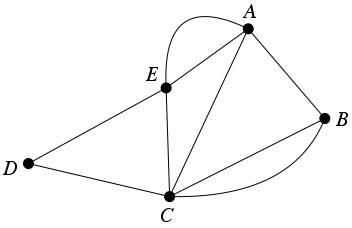
\includegraphics[width=6 cm]{asset/graph.jpg}
\end{figure}
\end{frame}

\begin{frame}
\frametitle{Mengenal Graph (lanj.)}
Melalui ilustrasi diatas, dapat disimpulkan bahwa edge memiliki fungsi untuk menghubungkan antar-node. \alert{Degree} sebuah node didefinisikan sebagai jumlah edge yang terhubung pada node tersebut.\newline\newline
Pada contoh graph di atas, maka degree node A adalah 4, degree node B adalah 3, dan seterusnya. Degree node dalam graph bisa berapa saja, tidak seperti binary search tree yang pasti hanya dapat memiliki maksimal 2 anak dan 1 parent. 
\end{frame}

\begin{frame}
\frametitle{Jenis-jenis Graph}
Berdasarkan hubungan antar node, graph terbagi menjadi 2:
\begin{itemize}
	\item Directed graph, yaitu graph satu arah. Di graph jenis ini, jika terdapat edge dari A ke B, maka belum tentu terdapat edge dari B ke A. Contoh graph ini adalah kota-kota sebagai nodenya dan jalan 1 arah sebagai edgenya.
	\item Undirected graph, yaitu graph dua arah. Dalam graph ini, jika terdapat edge dari A ke B, maka pasti juga terdapat edge dari B ke A. Contoh graph jenis ini adalah kota-kota sebagai nodenya dan jalan 2 arah sebagai edgenya.
\end{itemize}
\end{frame}

\begin{frame}
\frametitle{Jenis-jenis Graph (lanj.)}
Berdasarkan bobot dari edgenya, graph juga terbagi menjadi 2:
\begin{itemize}
	\item Unweighted Graph, yaitu graph yang mana edgenya tidak memiliki value, sehingga semua edge memiliki weight 1 dan hanya bermakna bahwa memang terdapat hubungan antar node yang dihubungkannya.
	\item Weighted Graph, yaitu graph yang mana edgenya memiliki bobot yang berbeda-beda. Bobot pada edge ini seringkali berupa biaya atau jarak yang harus ditempuh jika menggunakan edge tersebut.
\end{itemize}
\end{frame}

\begin{frame}
\frametitle{Representasi Graph pada Pemrograman}

Graph dapat direpesentasikan dalam pemrograman menggunakan 2 metode, yaitu adjacency matrix dan adjacency list.
\end{frame}

\begin{frame}
\frametitle{Adjacency Matrix}

Pada adjacency matrix, kita harus menyediakan array 2 dimensi dengan ukuran N x N yang mana N merupakan banyaknya node/vertex. \newline\newline
Awalnya, seluruh elemen matrix berisi nilai 0 yang menandakan bahwa tidak terdapat edge. Pada unweighted graph, jika terdapat edge dari node A ke node B, maka kita ganti isi dari $matrix[A][B] = 1$. Misal pada weighted graph dan terdapat edge dari A ke B dengan bobot C, maka update $matrix[A][B] = C$.
\end{frame}

\begin{frame}
\frametitle{Adjacency List}

Pada adjacency list, graph disimpan dalam array of lists. Tiap list berisi keterangan mengenai edge yang terdapat dalam suatu node. Ukuran dari array merupakan N yang mana N merupaka banyaknya node/vertex. \newline\newline
Awalnya, seluruh list tidak memiliki isi yang menandakan bahwa belum terdapat edge dalam graph tersebut. Pada unweighted graph, jika terdapat edge dari node A ke node B, maka, masukkan B kedalam list A. Pada weighted graph, jika terdapat edge dari node A ke node B dengan bobot C, maka masukkan \{B,C\} kedalam list A. Di sini isi dari list terdapat 2 item, yaitu node yang dituju beserta bobotnya
\end{frame}


\begin{frame}[fragile]
\frametitle{Pseudocode Representasi Graph}

Adjacency Matrix
\begin{lstlisting}
	integer AdjMatrix[N][N]
	set AdjMatrix = 0
	
	<@\textcolor{mygreen}{//edge dari 1 ke 4 pada undirected unweighted graph}@>
	AdjMatrix[1][4] = 1
	AdjMatrix[4][1] = 1
\end{lstlisting}
Adjacency List
\begin{lstlisting}
	List<integer> AdjList[N]
	
	<@\textcolor{mygreen}{//edge dari 1 ke 4 pada undirected unweighted graph}@>
	AdjList[1].push(4)
	AdjList[4].push(1)
	
\end{lstlisting}
\end{frame}

\begin{frame}
\end{frame}

\end{document}